\documentclass{beamer}
\usepackage[utf8]{inputenc}
\usepackage{amsmath}
\usepackage{enumitem}
\usepackage{graphicx}
\usepackage{amsmath}
\usepackage{listings}
\usetheme{Szeged}
\usecolortheme{beaver}

\title{Randomization-Based Inference}
\subtitle{Math 420}
\author{Riley Coburn \& Jake Caldwell}
\institute{Denison University}

\begin{document}

\begin{frame}
\titlepage
\end{frame}

\begin{frame}{}
    \begin{figure}[htp]
        \centering
        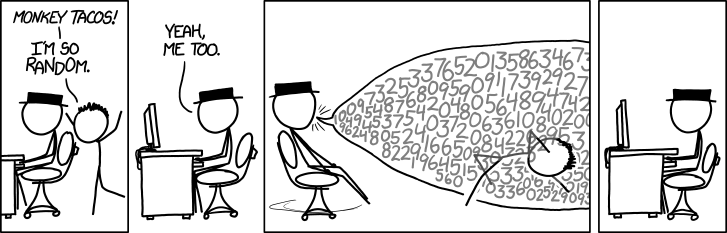
\includegraphics[width=10cm]{class9 random.jpg}
    \end{figure}
\end{frame}

\begin{frame}{\textbf{Road Map}}
    \begin{itemize}
    
        \item[$\blacksquare$] Review of Randomization Based Inference
        
        \item[$\blacksquare$] Introduction to the Theory of RBI
        
        \item[$\blacksquare$] Example Problem
        
        \item[$\blacksquare$] The Benefits of RBI
        
        \item[$\blacksquare$] A word about Monte Carlo Tests
        
    \end{itemize}
\end{frame}

\begin{frame}{\textbf{What is Randomization-Based Inference}}
    
    Randomization-based inference is a non-parametric tool that allows us to perform inference on sample populations that don't meet distribution assumptions.
    
\end{frame}

\begin{frame}{\textbf{What is Randomization-Based Inference}}
    
    Essentially, we leave the x-variable(s) alone and scramble the y-variable values. We then extract our desired statistic and repeat this process thousands to tens of thousands of times. 
    
    \begin{figure}[htp]
        \centering
        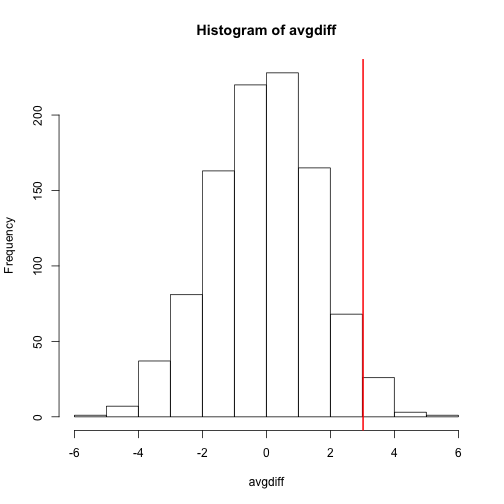
\includegraphics[width=5cm]{permutation_tests-diff_hist-1.png}
    \end{figure}
    
\end{frame}

\begin{frame}{\textbf{Formalism}}
    
    \newline\quad
    
    Let $\Gamma$ be our sample statistic. For each permutation, we compute a new test statistic, $\gamma_i$ for which we will then compute the ratio:
    
    $$\dfrac{\sum\limits_{i=1}^{n}\gamma_i}{n}\quad\forall (\gamma_i\geq\Gamma)$$
    
    \begin{center}
        This ratio is our theoretical p-value.
    \end{center}
    
\end{frame}

\begin{frame}{\textbf{Why Does This Work?}}

    We can equate a Randomization Based Inference to a permutation test. This is due to the re-sampling nature of RBI.
    
    \newline\quad
    
    We equate these two concepts because a permutation is one way that data can be arranged. As we previously mentioned, we rearrange the y-variable N times, which results in N permutations. 
    
    $$
        \begin{pmatrix}
            x_{1,1} & x_{1,2} & \cdots & y_{1,n} \\
            x_{2,1} & x_{2,2} & \cdots & y_{2,n} \\
            \vdots  & \vdots  & \ddots & \vdots  \\
            x_{n,1} & x_{n,2} & \cdots & y_{n,n} 
        \end{pmatrix}\longrightarrow
        \begin{pmatrix}
            x_{1,1} & x_{2,2} & \cdots & y_{i,n} \\
            x_{2,1} & x_{2,2} & \cdots & y_{i,n} \\
            \vdots  & \vdots  & \ddots & \vdots  \\
            x_{n,1} & x_{n,2} & \cdots & y_{i,n} 
        \end{pmatrix} 
    $$
    \begin{center}
        For $i\in \{1,2,3\dots,n\}$ for N-many permutations.
    \end{center}
\end{frame}

\begin{frame}{\textbf{Why Does this Work?}}

    RBI has a unique property. They are considered an approximation of an exact test. 
    
    \newline\quad
    
    An exact test is a type of statistical significance test in which the distribution of the test statistic under the null hypothesis is obtained by calculating all possible values of the test statistic under all possible rearrangements of the observed data points.
    
\end{frame}

\begin{frame}{\textbf{Exact Tests and the CLT}}

    We base the sample size condition for a lot of our models and tests around the Central Limit Theorem. 
    
    \newline\quad
    
    We can also use the Central Limit Theorem to get an asymptotically correct p-value from the statistic distribution created from a RBI. This is because the more permutations we have, the better estimated distribution we will have for to conduct hypothesis testing on.
    
\end{frame}

\begin{frame}{\textbf{Exact Test Explanation}}
    
    Suppose that $T_n(X,\dots,X_n)$ is a given test statistic $T_n:\Omega^n\rightarrow\mathbb{R}$ based on $\Omega$-valued random variables. In practice often a central limit theorem holds for $T_n$ under $H_0$ and a consistent variance estimator $V_n$, for its unknown asymptotic variance is available. Then the one-sided upper $T_n$-test $\psi_n$ for $H_0$ can be carried out as asymptotic level $\alpha$.
    
\end{frame}

\begin{frame}{\textbf{Deeper Dive}}

    If we had access to all permutations of the data, we could produce an exact p-value as in an exact test. This could happen if we wanted to determine if we had a fair coin and flipped the coin 3 times ($2^3=8$) but not if we flipped the coin 100 times ($2^{100}=1.267\cdot10^{30}$)
    
    \newline\quad
    
    However, there is a solution to the latter situation. We will apply the Monte Carlo Test. We will cover this at the end of the presentation.
    
\end{frame}

\begin{frame}{\textbf{Example}}

    Suppose we want to use ANOVA to determine if there is a difference in the survival rate of 5 different types of cancers. However, this model does not satisfy the normality and equal variance condition. 
    \begin{figure}
        \centering
        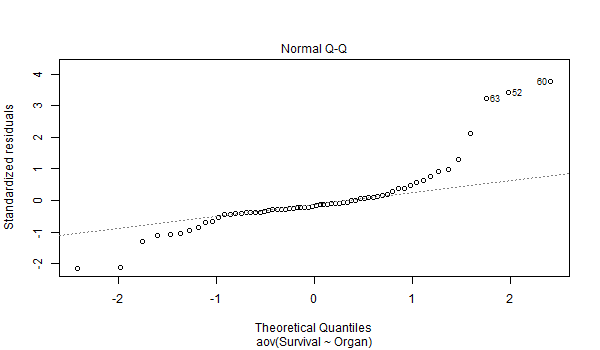
\includegraphics[width = 5cm]{NormalQQ.png}
        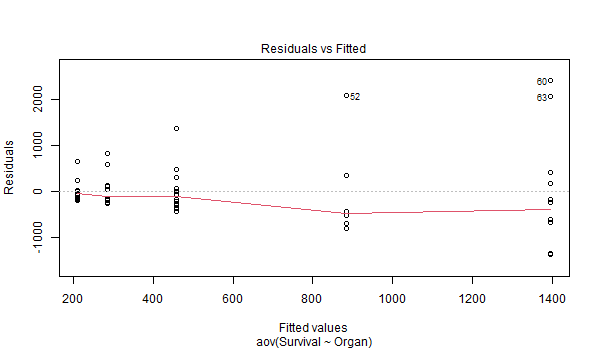
\includegraphics[width = 5cm]{ResidvsFitted.png}
    \end{figure}
\end{frame}

\begin{frame}{\textbf{Example}}
    The good thing about this model, however, is that when the Bartels Test for Randomness is ran on it, it has a ($p = 0.3$). This means we fail to reject that the data is random. We can proceed with a randomization based inference on the F-statistic.
    
\end{frame}

\begin{frame}[fragile]{\textbf{Example}}
We can do the following:
\newline\quad
    \begin{lstlisting}[language = R]
        ```{r}
        mod=lm(Survival~Organ,data=Cancer)
        anova(mod)
        res=anova(mod)$"F value"
        t=do(1000)*(anova(lm(shuffle(Survival)~
        as.factor(Organ),data=Cancer))$"F value")
        ```
    \end{lstlisting}
    \newline\quad
This will extract 1000 different F-statistics from 1000 different permutations of the Cancer Data

\end{frame}

\begin{frame}{\textbf{Example}}
Which yields this estimate F-Distribution
     \begin{figure}
        \centering
        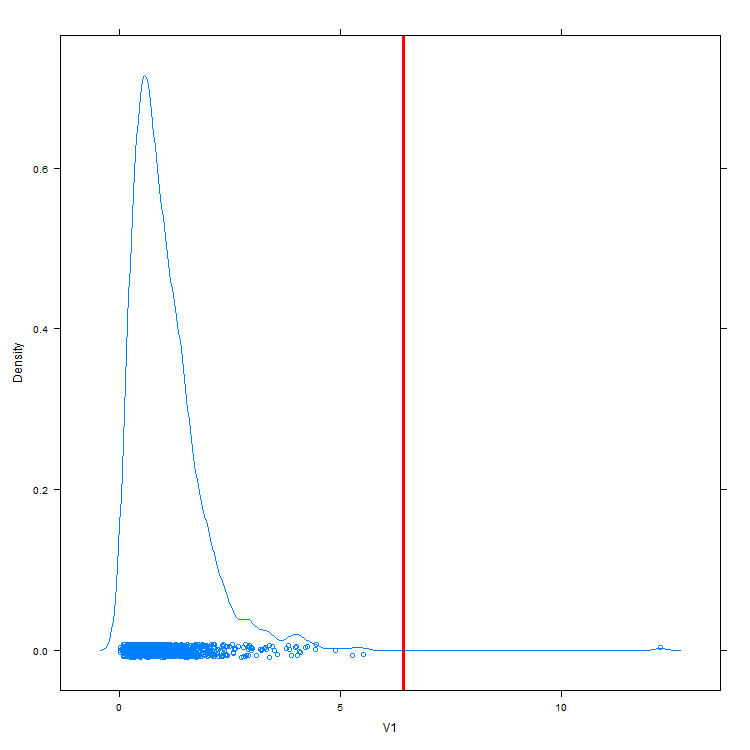
\includegraphics[width = 5cm]{DensityPlot.png}
    \end{figure}
The red line is our original observed F-stat
\end{frame}
\begin{frame}{\textbf{Example}}
    From that figure, we can generate our asymptotically correct P-value by doing $\frac{F-Stats \geq{6.43344}}{1000}$, which is $p = .001$. 
    This p-value we can trust because we have generated enough permutations to have an approximate exact test with an error rate fixed at .05. 
\end{frame}
\begin{frame}{\textbf{Benefits of Randomization Based Inference}}
    \begin{itemize}
    
        \item[$\blacksquare$] Makes abstract p-values into simple proportions, $\frac{Num Stats \geq{Observed Stat}}{NumPermutations}$ 
        
        \item[$\blacksquare$] It is non-parametric, so it doesn't have the same constraints as models or tests
        
        \item[$\blacksquare$] P-values are exact when we know all possible permutations
        
        \item[$\blacksquare$] Can be generalized to a wide variety of statistics
        
        \item[$\blacksquare$] Rooted in the CLT, which can be easily explained
        
    \end{itemize}
\end{frame}
\begin{frame}{\textbf{Possible Limitations}}
\begin{itemize}
    
        \item[$\blacksquare$] Data has to be random
        
        \item[$\blacksquare$] Could be computationally expensive depending on number of permutations
        
        \item[$\blacksquare$] Doesn't allow us to easily generate confidence intervals for statistics
        
    \end{itemize}
    
\end{frame}
\begin{frame}{\textbf{A Word about Monte Carlo Testing}}
A Monte Carlo test can generate an exact P-value when the total number of permutations are too large by taking a random sample of N permutations. It then generates a "reference distribution". 

\newline\quad
\newline\quad

For clarification, you can think of this as a bridge between a true permutation test and randomization based inference. 

\newline\quad
\newline\quad

This can also be used to tackle small sample sizes, we will touch on this more in our paper.  
\end{frame}
\end{document}

